\subsection{Supervised Baselines on the Preserved Test Sets}
\label{sec:supervised}

The classifier controls use the splits and settings in
Section~\ref{sec:supervised_methods}.
Table~\ref{tab:supervised} summarises the learning curve and the
DistilBERT results at both training-label budgets.
The 20,000-record encoder fits take approximately 80~s each and peak
at 1.30~GiB allocated memory; their warm serial inference averages
2.07~ms on the same workstation used for the HF adaptation benchmark.

\begin{table}[tb]
\centering
\caption{Supervised balanced-test performance. F1 is computed on the
pooled 3,000 records; DistilBERT values average three separate model fits.
Every row uses 2,000 additional validation labels; total labelled budgets
are training records plus 2,000. Latency is warm serial end-to-end feature/token preparation and inference.}
\label{tab:supervised}
\begin{tabular}{lrrr}
\toprule
Model & Training records & Weighted F1 & Latency (ms) \\
\midrule
TF-IDF/SVM (CPU) & 500 & 0.7546 & 0.29 \\
TF-IDF/SVM (CPU) & 2,000 & 0.7908 & 0.29 \\
TF-IDF/SVM (CPU) & 10,000 & 0.8241 & 0.28 \\
TF-IDF/SVM (CPU) & 20,000 & 0.8291 & 0.29 \\
DistilBERT (3 epochs) & 500 & $0.5329\pm0.1522$ & 2.06 \\
DistilBERT (early stop) & 500 & $0.7150\pm0.0208$ & 2.07 \\
DistilBERT (GPU) & 20,000 & $0.8244\pm0.0046$ & 2.07 \\
\botrule
\end{tabular}
\end{table}

Paired two-sided McNemar comparisons against the Gemma~4 GGUF zero-shot
balanced predictions (Table~\ref{tab:results_balanced}) give
Holm-adjusted $p<0.001$ for the 20,000-record
SVM and for each of the three 20,000-record DistilBERT fits,
with positive accuracy differences of 4.67--5.60 percentage points for
these encoder fits. Correction covers all 42
baseline--reference--condition comparisons. This tests accuracy gains,
not F1 differences; the zero-shot and supervised label budgets differ.

Figure~\ref{fig:label_budget} shows the observed training-budget trade-off.
At 500 training records, adapter mean F1 exceeds the label-matched SVM
point estimate. At 2,000 training records, SVM reaches 0.7908, above the
three observed 500-record adapter means, with warm CPU latency below
0.3~ms. This latter comparison uses different total label budgets
(4,000 versus 2,500). The LLM learning curve and a crossover budget
remain unmeasured; these observations do not establish a threshold
beyond which adaptation is unnecessary.

\begin{figure}[tb]
\centering
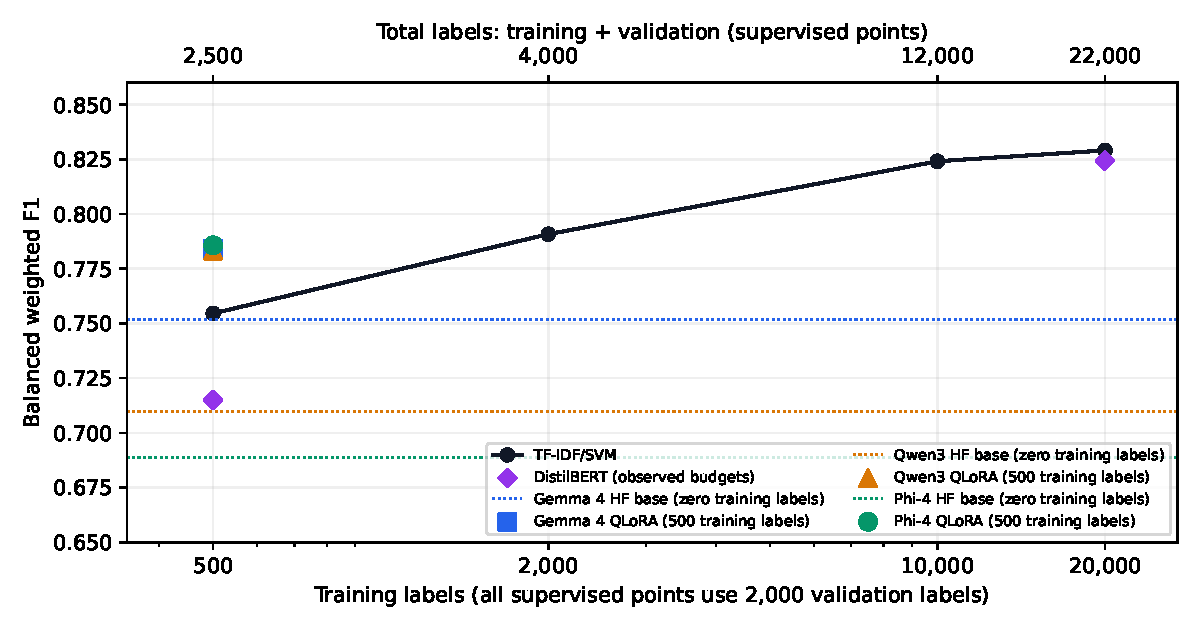
\includegraphics[width=\textwidth]{figures/v2/label_budget_tradeoff.pdf}
\caption{Observed balanced 500-character weighted F1 by training-label
budget (log axis). Direct classifiers additionally use 2,000 validation
labels; the upper axis shows their total annotation requirement. QLoRA
points use 500 training plus 2,000 validation labels. DistilBERT and
QLoRA points are means over three fits; no unmeasured intermediate
encoder or LLM budgets are interpolated. Horizontal HF base references
use zero task-labelled training data and the fixed thinking-off protocol.}
\label{fig:label_budget}
\end{figure}

These supervised comparisons use additional labelled data and
therefore measure a different deployment regime from zero-shot
inference. Their strong performance requires the LLM deployment
recommendations to be conditional on the availability of training
labels. The matched 500-training-label LLM adaptation experiment is
reported in Section~\ref{sec:qlora_results}; higher-budget baselines do not establish equal-budget
superiority. All supervised budgets additionally use the same 2,000
validation labels.
